\documentclass[11pt]{article}
\usepackage{graphicx}
\usepackage[bookmarks=true]{hyperref}
\usepackage{bookmark}
\usepackage{hyperref}
\usepackage{csquotes}
\usepackage{float}
\usepackage{wrapfig}
\usepackage{array}
\usepackage{wrapfig}
\usepackage[justification=justified,singlelinecheck=false]{caption}
\newcolumntype{L}[1]{>{\raggedright\let\newline\\\arraybackslash\hspace{0pt}}m{#1}}
\newcolumntype{C}[1]{>{\centering\let\newline\\\arraybackslash\hspace{0pt}}m{#1}}
\newcolumntype{R}[1]{>{\raggedleft\let\newline\\\arraybackslash\hspace{0pt}}m{#1}}

\setlength{\parindent}{0pt}

\begin{document}
\begin{titlepage}
\begin{flushright}


\includegraphics[width=380px]{../global/University_of_Pretoria_Logo.png}
\newline
\newline

\textbf {\LARGE Plan for Software Aspects of Certification} \newline

\textbf {\Large (PSAC)} \newline

\centering
\includegraphics[width=100px]{../global/Logo.jpg}

\textbf {\Large Linphone for Android Group Chat (Waterfall)}\newline

\flushright \textbf {\large Version: 1.2}\newline

\centering \textbf {\large Authors:}

\begin{table}[H]
\large
\centering
\begin{tabular}{rl}
	Izak Blom & 13126777 \\
	David Breetzke & 12056503 \\
	Paul Engelke & 13093500 \\
	Prenolan Govender & 13102380 \\
	Jessica Lessev & 13049136 \\
\end{tabular}
\end{table}

Date: \today

\end{flushright}
\end{titlepage}

\setcounter{tocdepth}{3}
\setcounter{secnumdepth}{5}
\tableofcontents

\newpage
\section{Systems Overview} 
Linphone Android was extended to provide group chat functionality. This gives a user the ability to create, delete, participate in and manage group chats. This enables numerous users to collaborate/communicate simultaneously with each other. Linphone group chat functionality provides the option for secure communication between parties through encryption of messages.

\section{Systems Configuration}
\subsection{Minimum Device Requirements}
A mobile device with an Android operating system, such as
\begin{itemize}
\item smart phones,
\item and tablets.
\end{itemize}
%\textbf{For compilation:} A computer with a Linux operating system is required.
\subsection{Minimum Software Requirements}
An Android operating system of 2.2 or higher.\\
%\textbf{For installation:} Require a computer with Linux operating system.
%\begin{itemize}
%\item Make sure that you have Eclipse IDE installed on your Linux environment.
%\end{itemize}

\subsection{Communication}
\begin{figure}[H]

\includegraphics[width=300px]{./images/network.png}
\caption{Linphone system configuration}
\label{Configuration}
\end{figure}


\newpage
\section{Installation}
To install the application make sure that you are in a Linux environment with the Eclipse IDE installed.
To install the Linphone application simply follow the steps below:
%\begin{enumerate}
%\item Locate your Android device's Play store
%\item Under the search tab, search for "Linphone"
%\item Locate the Linphone application and click on it
% 
\includegraphics[width=10px]{./images/icon.jpg}
%\item Follow your device's guidelines to install the application
%\item Once installed, launch the application by clicking on the Linphone icon which should be %listed in the applications list on your device.
%\item Once launched, follow the prompts to register if you are a new user or to log in if you %already have an account.
%\end{enumerate}
\begin{enumerate}
\item Locate the repository - \url{https://github.com/psengelke/linphone-android-group-chat.git}
\begin{figure}[H]
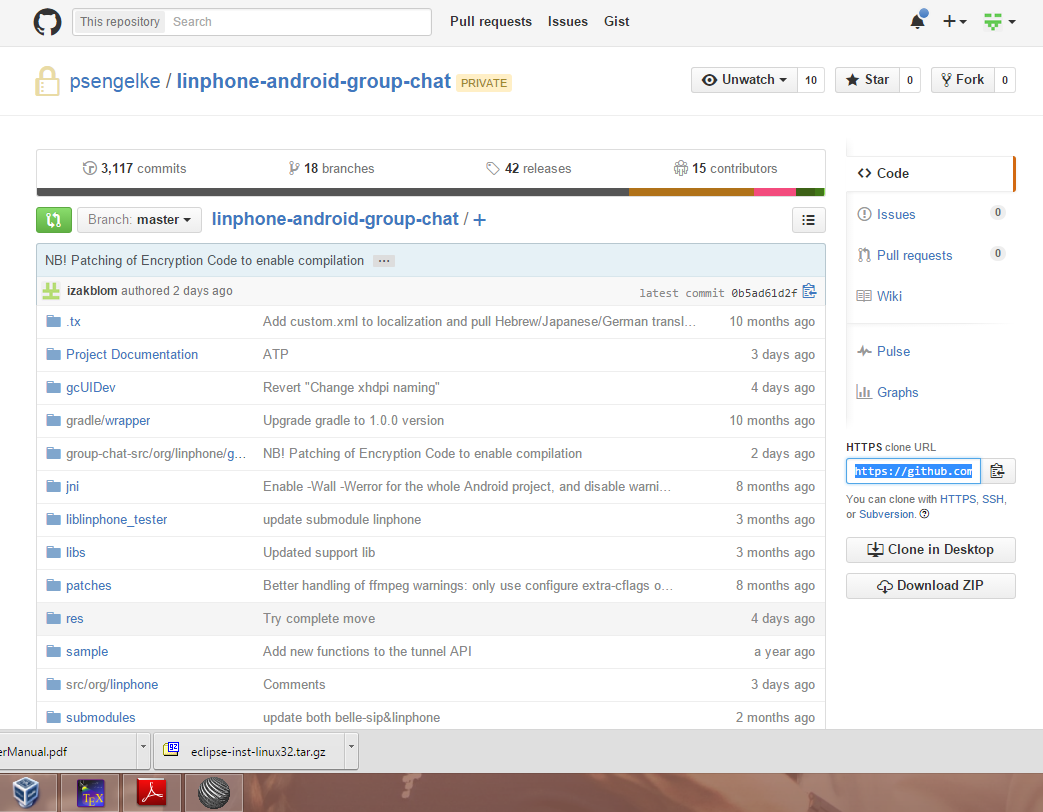
\includegraphics[width=100px]{./images/repoLocate.png}
\caption{Locate repository}
\label{repoLocate}
\end{figure}
\item Here there are two separate ways to go about installing the application. Using an IDE or using a makefile. 
\end{enumerate}

\textbf{Using Eclipse IDE}
\begin{enumerate}
\item Navigate to directory where you wish to clone the repository. 
\item Clone the repository to your local hard disk by typing the following command in the terminal: "git clone https://github.com/psengelke/linphone-android-group-chat.git" 
\item Navigate to the cloned repository in your directory. Refer to figure 3
\item Pull all the submodules by typing the following command in the terminal: "git submodule update --init --recursive". Refer to figure 3
\begin{itemize}
\item Note: This may take several minutes. 
\item Refer to figure 3.
\end{itemize}
\begin{figure}[H]
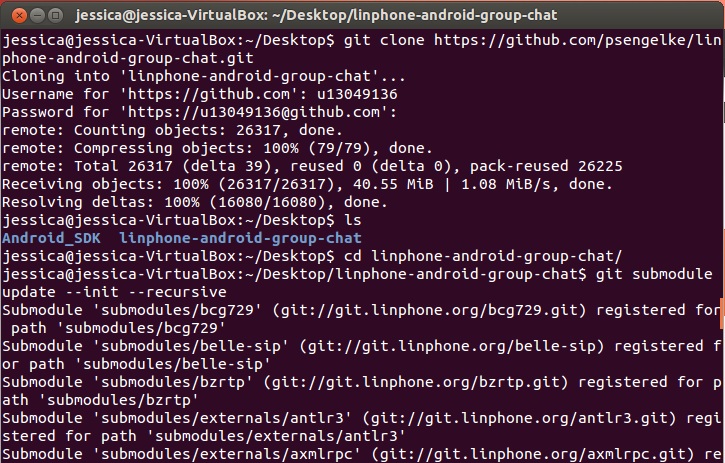
\includegraphics[width=100px]{./images/clone.png}
\caption{Clone repository and pull submodules}
\label{repoClone}
\end{figure}
\item Open the Eclipse IDE
\item Click File -$>$ Import -$>$ Git -$>$ Projects From Git -$>$ Next -$>$ Existing local repository -$>$ Locate the newly cloned repository and add it -$>$ Import existing Eclipse projects -$>$ Next -$>$ Check Projects -$>$ Finish
\subitem The project will appear at the bottom left hand corner.
\begin{figure}[H]
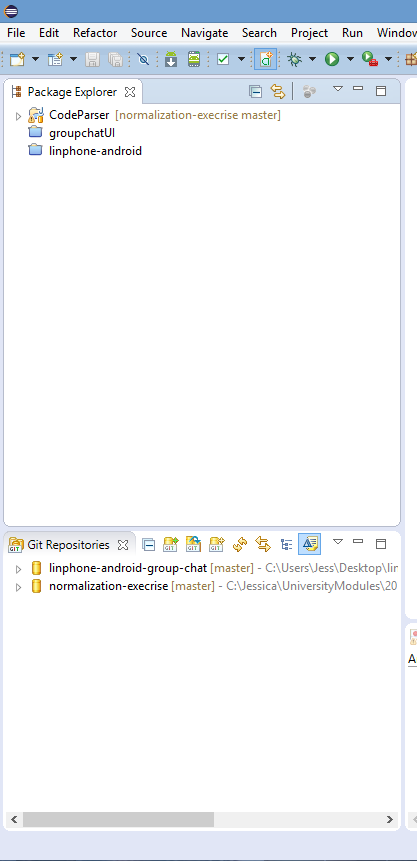
\includegraphics[width=100px]{./images/git.png}
\caption{Clone repository to Eclipse IDE}
\label{repoClone}
\end{figure}
\item \textbf{Setup Device: } Set device to Developer Mode through the settings. 
\subitem Settings -$>$ Developer Options -$>$ On
\subitem Enable debugging mode in developer options.
\subitem Plug device into your computer (USB port).
\subitem Install necessary device drivers if they are not already available on the computer.
\item Locate the green "Play" button on the top of the Eclipse IDE and select it.
\begin{figure}[H]
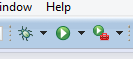
\includegraphics[width=80px]{./images/eclipsePlay.png}
\caption{Eclipse IDE Play}
\label{repoClone}
\end{figure}
\item A prompt will appear, with the options to select which device you would like to run the application on. Select the desired device.
\begin{figure}[H]
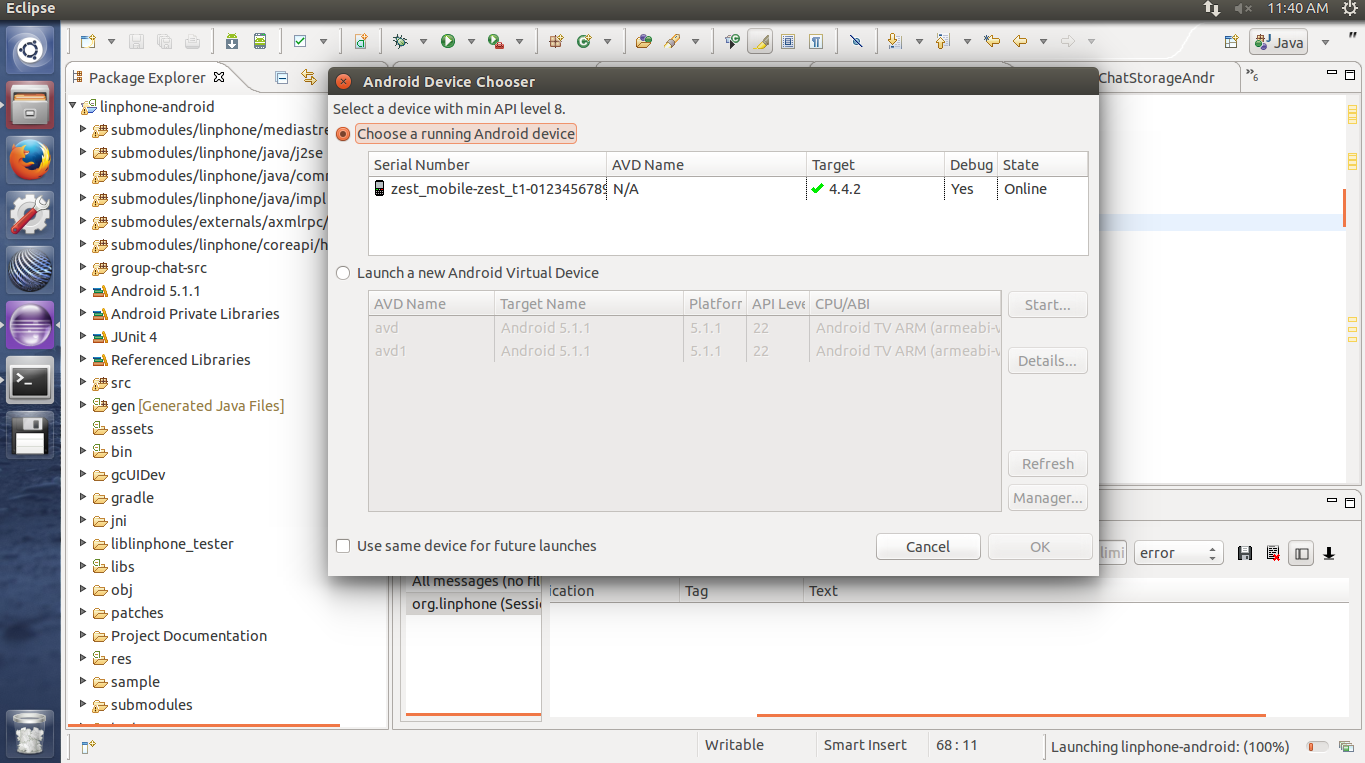
\includegraphics[width=150px]{./images/ChooseDeviceScreenShot.png}
\caption{Eclipse IDE Play}
\label{repoClone}
\end{figure}
\item The application will be launched on your selected device.
\end{enumerate}

\textbf{Using a Makefile}
\begin{enumerate}
\item Download the Android sdk with platform-tools and tools updated to latest revision (at least API 16 is needed), then add both 'tools' and 'platform-tools' folders in your path.
\item Download the Android ndk (=r10c) from Google and add it to your path.
\item Install yasm, nasm, curl, ant, rsync and the autotools: autoconf, automake, aclocal, libtoolize, pkgconfig.
\subitem On 64 bits linux systems you'll need the ia32-libs package
\subitem With the latest Debian (multiarch), you need this:
\subsubitem dpkg --add-architecture i386
\subsubitem aptitude update
\subsubitem aptitude install libstdc++6:i386 libgcc1:i386 zlib1g:i386 libncurses5:i386
\item run the Makefile script in the top level directory. This will download iLBC source files and convert some assembly files in VP8 project.
\begin{verbatim}$ make \end{verbatim}
\item To generate a signed apk to publish on the Google Play, run  \begin{verbatim} $ make release \end{verbatim}
\item Locate the created APK on the the computer and copy it onto the device. 
\item Locate device on device - select it and follow the prompts.
\end{enumerate}

\section{Getting Started}
%In order to make use of the application one needs to have a linphone.org account and SIP account. %Follow the steps below to create one:
%\begin{enumerate}
%\item Launch the application
%\item Click the "Start" button located on the bottom right of the screen
%\item Click on "Create an account on linphone.org" if you are a new user 
%\subitem Follow the prompts on the screen to create an account
%\item Click on "I have already a linphone.org account" if you already have an account
%\subitem Enter the neccessary account information and click "Sign in"
%\item Click on "I already have an SIP account" if you already have a SIP address to use
%\subitem Enter the neccessary account information and click "Sign in"
%\item Once logged in you will be presented with the application user interface
%\end{enumerate}
In order to make use of the application one needs to have a linphone.org account and SIP account. Make sure that all members that you wish to add to a group chat, if you are creating a group chat, also have the necessary accounts.
\subsection{Using the Group Chat functionality}
Below is a diagram showing how one can navigate through the interfaces involved in the group chat functionality. \\
\begin{figure}[H]
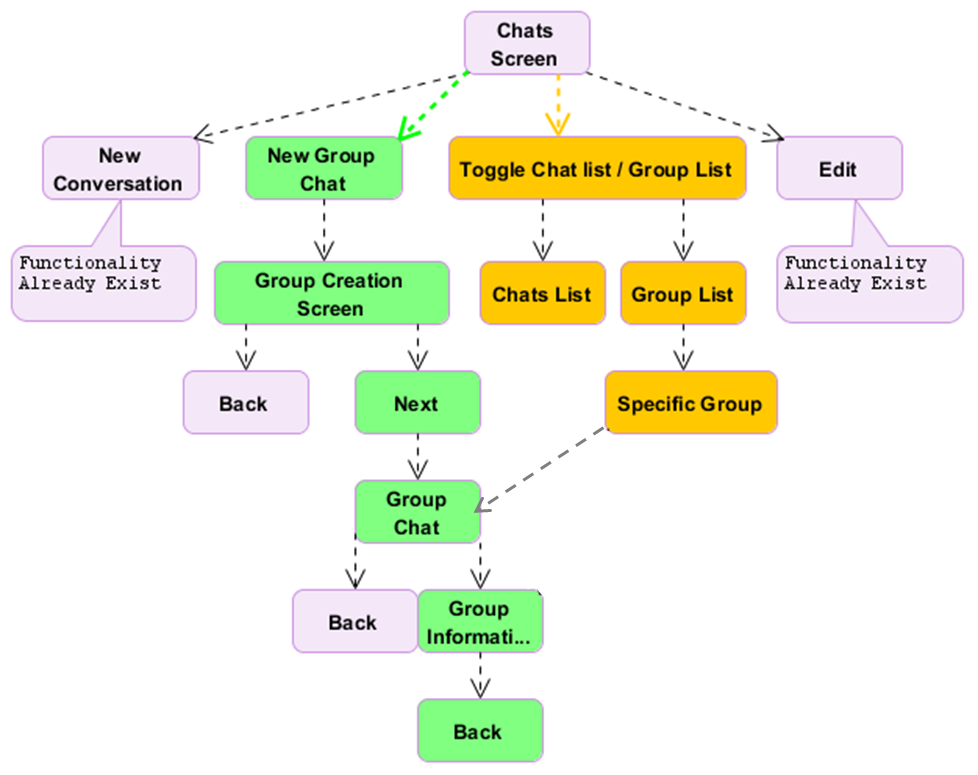
\includegraphics[width=300px]{./images/flow.png}
 \caption{Image showing navigation throughout system}
 \label{flow}
 \end{figure}



\section{Using The System}


\subsection{Guidelines}
When viewing the "Chat" user interface, one will be presented with the following options on the top panel of the screen:
\begin{itemize}
\item New Conversation
\item New Group Chat
\item Edit
\end{itemize}
Below are guidelines on how to use the system. Guidelines are provided for various sections. The sections covered by the guidelines are as follows:

\begin{itemize}
\item Locate list of group chats \ref{locate}
\item Create new group chat. \ref{create}
\item Chat in the group chat \ref{chat}
\item View group chat information \ref{info}
\item Edit existing group chat. \ref{edit}
\item Add/remove members from existing group chat. \ref{add}
%\item Green Path - from the flow diagram.
%\item Orange Path - from the flow diagram. 
\end{itemize}

\subsubsection{Locate list of group chats} \label{locate}
Follow the steps below to locate the location/list of all your current group chats:
\begin{enumerate}
\item Start the application
\item On the "Home" screen click the "Chat" option as shown in the diagram\\
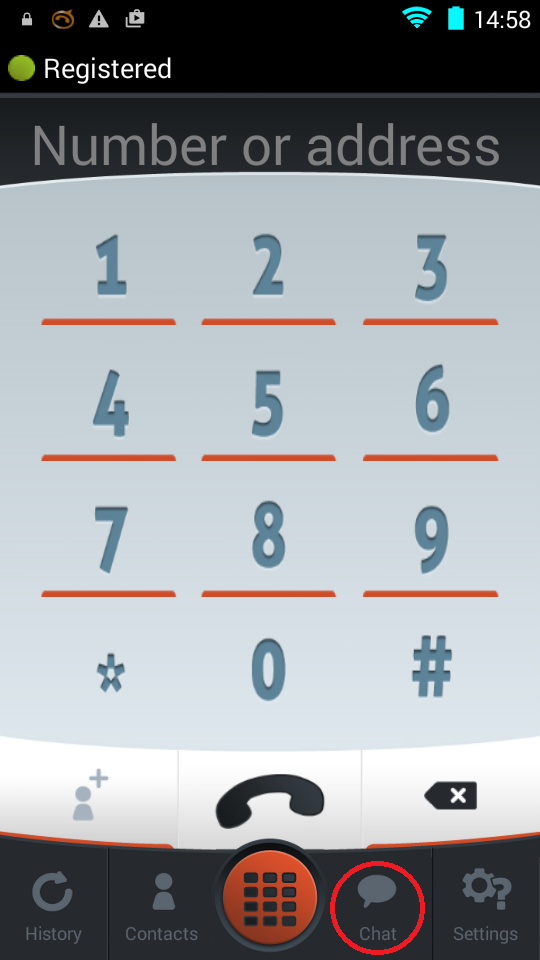
\includegraphics[width=50px]{images/mainScreen.png}
\item Click on the "Groups" button\\

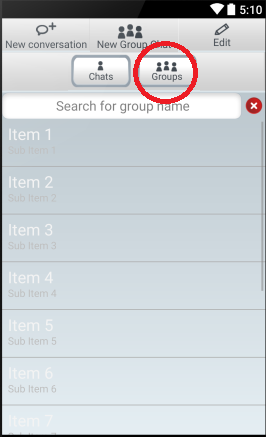
\includegraphics[width=50px]{images/ChatlistNav.png}
\item You are now presented with the list of group chats
\begin{enumerate}
\item If a group chat from the list is selected, the group chat will open\\
\end{enumerate}
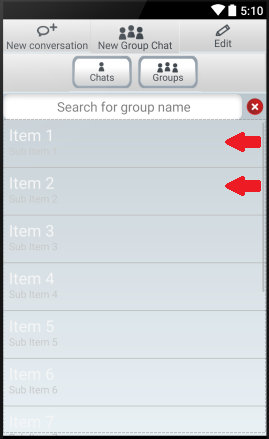
\includegraphics[width=50px]{images/Grouplist.png}
\item to navigate back to your private chat lists, click on the "Chats" button\\
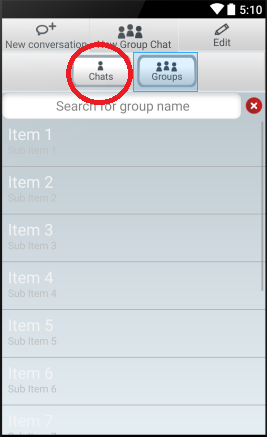
\includegraphics[width=50px]{images/GrouplistNav.png}
\end{enumerate}

\subsubsection{Create New Group Chat} \label{create}
Follow the steps below to create and launch a new group chat:
\begin{enumerate}
\item Start the application
\item On the "Home" screen click the "Chat" option as shown in the diagram\\
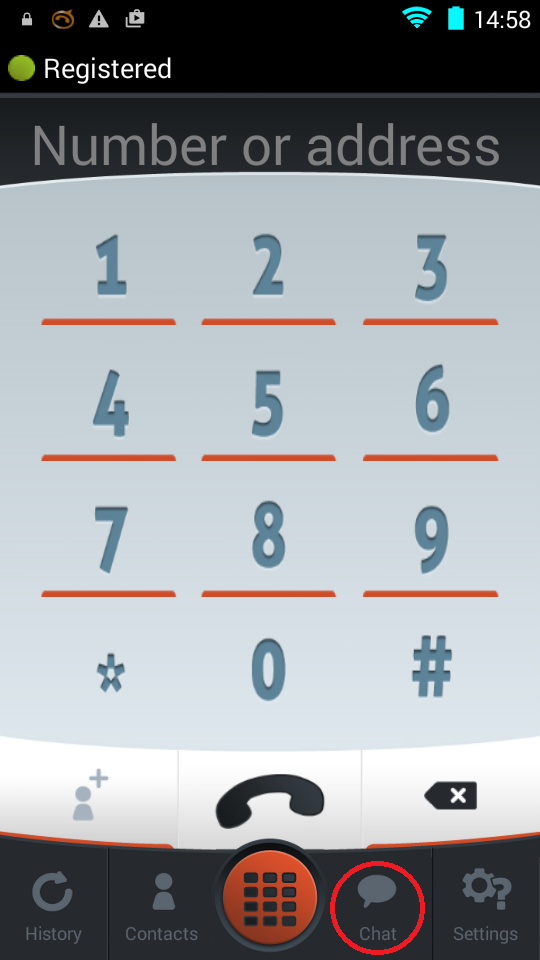
\includegraphics[width=50px]{images/mainScreen.png}
\item Click on the "New Group Chat" button\\
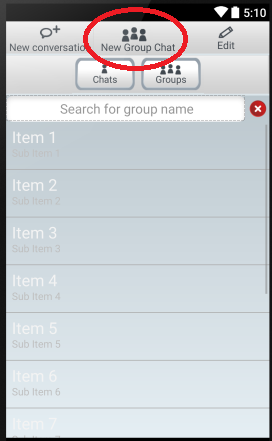
\includegraphics[width=50px]{images/ChatlistCG.png}
\item You are now presented with a user interface where necessary information is needed in order to create the group chat
\begin{enumerate}
\item Enter a desired group name
\item Choose the type of encryption you wish to use
\item Add members to participate in the group chat - Note: at least two members must be added
\subitem Type the member's SIP address in the text edit
\subitem Click on the green "+" button
\subitem To clear the text edit click on the red "X" to the left of the text edit
\subitem To remove a added member click on the red "X" next to the corresponding member you wish to remove
\item Click "Next"
\end{enumerate}
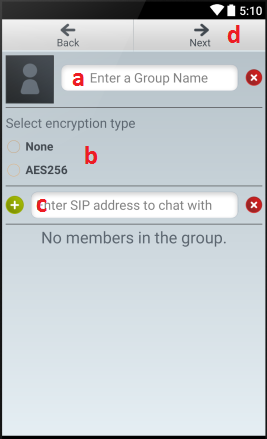
\includegraphics[width=50px]{images/GroupChatCreation.png}
\item You will now be presented with the actual group chat where you can proceed to chat with the members\\
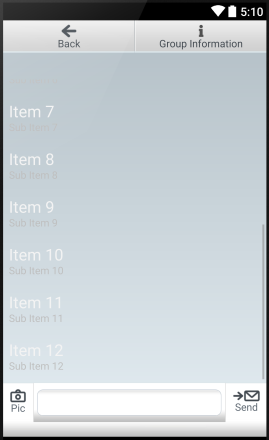
\includegraphics[width=50px]{images/groupchat.png}
\end{enumerate}

\subsubsection{Chat in Group Chat}  \label{chat}
Follow the steps below to participate in a group chat in which you are a member:
\begin{enumerate}
\item Start the application
\item On the "Home" screen click the "Chat" option as shown in the diagram\\
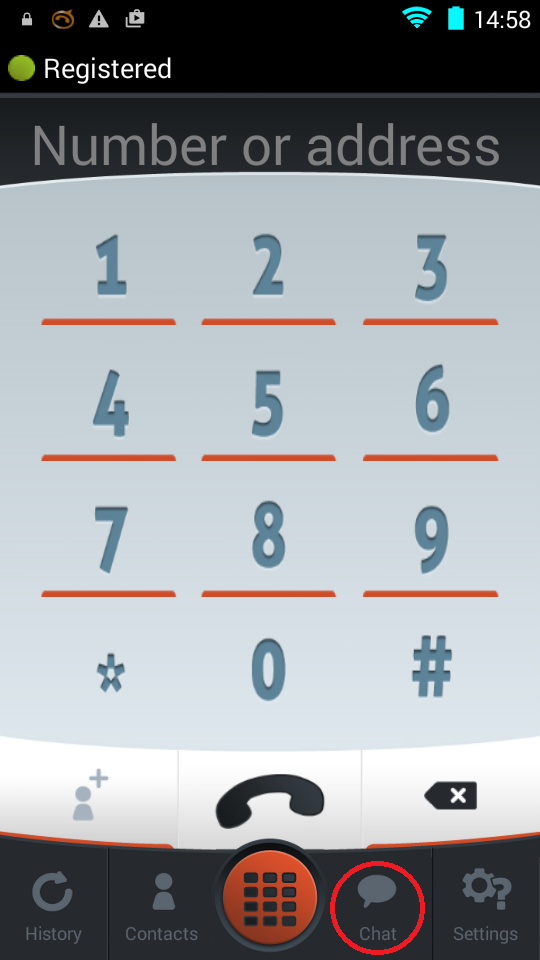
\includegraphics[width=50px]{images/mainScreen.png}
\item Click on the "Groups" button\\
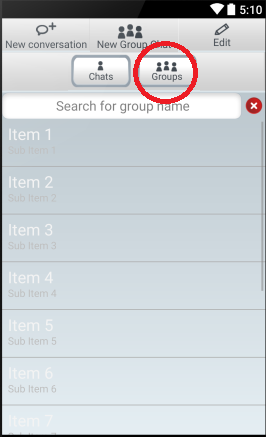
\includegraphics[width=50px]{images/ChatlistNav.png}
\item You are now presented with a list of the group chats in which you are a member and may participate
\item Click on the group chat in which you want to "chat"/participate\\
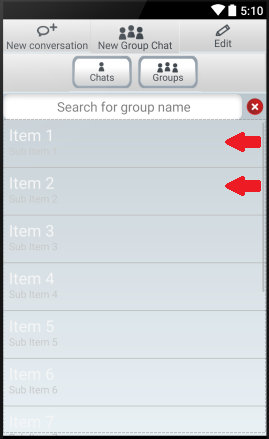
\includegraphics[width=50px]{images/Grouplist.png}
\item You will be presented with the group chat interface\\
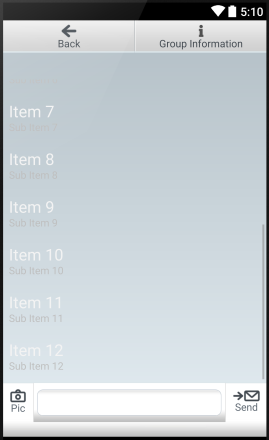
\includegraphics[width=50px]{images/groupchat.png}
\item To type a message:
\begin{enumerate}
\item Click on the text edit\\
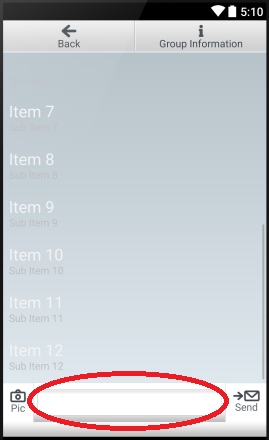
\includegraphics[width=50px]{images/groupchatEdit.png}
\item The keyboard will pop-up. Type the desired message
\item Click the "Send" button to send the message to the group and all the members in the group\\
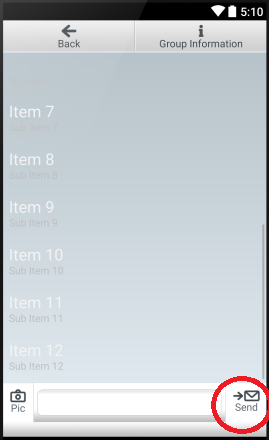
\includegraphics[width=50px]{images/groupchatSend.png}
\end{enumerate}
\item To send a picture/image to the group:
\begin{enumerate}
\item Click on the "Pic" button\\
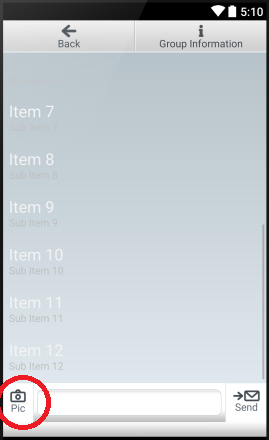
\includegraphics[width=50px]{images/groupchatSendPic.png}
\item You will be asked whether to send a picture already stored in you phone gallery or to take a new picture. Click on the button that corresponds to your desired choice.
\item Follow the respective steps for the picture option and select the image you wish to send
\item Once you locate the picture you wish to send, click on it and it will automatically send the the rest of the group members
\end{enumerate}
\end{enumerate}

\subsubsection{View Group Chat Information}  \label{info}
Follow the steps below to view a group chat's details and information:
\begin{enumerate}
\item Start the application
\item On the "Home" screen click the "Chat" option as shown in the diagram\\
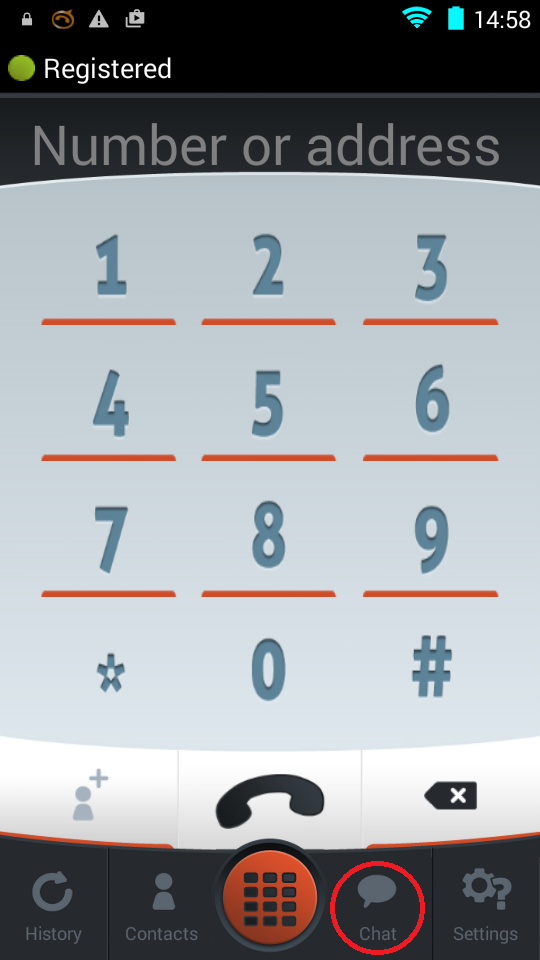
\includegraphics[width=50px]{images/mainScreen.png}
\item Click on the "Groups" button\\
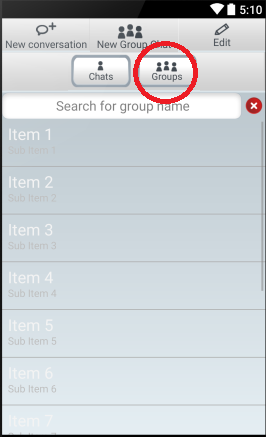
\includegraphics[width=50px]{images/ChatlistNav.png}
\item You are now presented with a list of the group chats
\item Click on the group chat for which you wish to see details\\
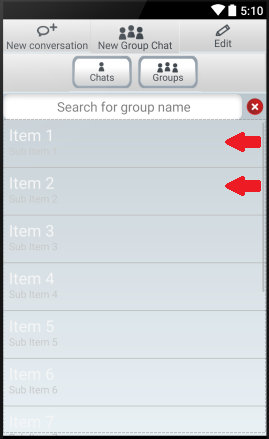
\includegraphics[width=50px]{images/Grouplist.png}
\item The actual group chat will open
\item Click on the "Group Information" button on the top right of the screen\\
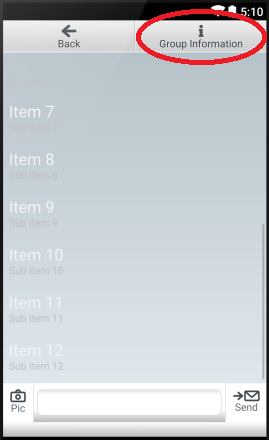
\includegraphics[width=50px]{images/groupchatInfo.png}
\item The groups information will be displayed\\
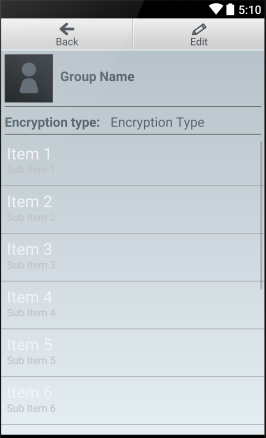
\includegraphics[width=50px]{images/groupchatInfoDisp.png}
\end{enumerate}

\subsubsection{Edit Existing Group}  \label{edit}
Follow the steps below to edit a group chat's details and information:
\begin{enumerate}
\item Follow the steps listed in the section \textbf{View Group Chat Information} to navigate to the group chat's information screen
\item Once on the group chat's information screen click on the "Edit" button\\
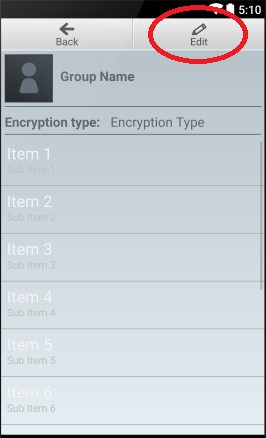
\includegraphics[width=50px]{images/groupchatInfoEdit.png}
\item The fields can be edited will be enabled
\begin{enumerate}
\item Click on the group name edit to change the group's name
\item Select a different encryption to use if desired by clicking on the radio button that corresponds to your choice
\item To add members to the group type the member's SIP address in the text edit
\item Click on the green "+" button
\item To clear the text edit click on the red "X" to the left of the text edit
\item To remove a added member click on the red "X" next to the corresponding member you wish to remove
\end{enumerate}
\item Click "Next"
\end{enumerate}


\subsubsection{Add/Remove Members from Existing Group}  \label{add}
Follow the steps below to add/remove members from a group chat:
\begin{enumerate}
\item Follow the steps listed in the section \textbf{Edit Existing Group} to navigate to the group chat's information screen and make the information editable
\item To add a member look at step \textbf{3c-e} under the \textbf{Edit Existing Group} section
\item To remove a member look at step \textbf{3f} under the \textbf{Edit Existing Group} section
\item Click "Next"
\end{enumerate}

%Looking at the diagram above, the steps to navigate through the user interface will be listed:
%\textbf{Green Path}
%\begin{enumerate}
%\item Once logged in you will be presented with the application user interface
%\item Click on the "Chat" menu item located on the bottom panel
%\item Click "New Group Chat" option located on the top panel
%\item You will be presented with a screen to enter necessary information to create a new group chat
%\subitem Enter a desired group name
%\subitem Choose the type of encryption you wish to use
%\subitem Add members to participate in the group chat - Note: at least two members must be added
%\subitem Click "Next"
%\item You will now be presented with the actual group chat
%\item You can now proceed to "chat" in the group chat or view the group information by clicking on "Group %Info" in the group chat
%\subitem You can edit the information by clicking "Edit" and changing the information desired.
%\end{enumerate}


\section{Troubleshooting}

For further problems not covered in this document please refer to the following link:
\url{http://www.linphone.org/user-guide.html}

\end{document}
